\chapter{\textbf{CHAPTER NAME}}
\label{chap:chapname}

\lipsum[1]

\section{\textbf{Section name format}} 
\label{sec:secname}

\lipsum[2-3]
\begin{figure}
\centering	
		\centering
		\subfloat[]{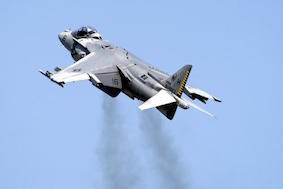
\includegraphics[scale=0.7]{figs/chap1/fig1.jpg} }
		\hspace{0.2cm}
		\subfloat[]{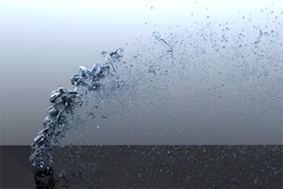
\includegraphics[scale=0.7]{figs/chap1/fig2.jpg} } \\
		\bigskip
\caption[Images from internet sites exemplifying physical conditions in which JICF configurations are detected]{\label{fig:jicf-examples}Images from internet sites exemplifying physical conditions in which JICF configurations are detected: (a) an AV-8B Harrier aircraft during vertical taking-off process; (b) atomization of an aircraft engine liquid fuel jet in a crossflow.}
\end{figure}

\lipsum[1-4]

\section{\textbf{Section name}}

Under the motivational aspects previously reviewed, this thesis:
\begin{itemize}
\item do A
\item do B and
\item do C
\end{itemize}


\section{\textbf{Citations}}

Special contents about JICF are found in Karagozian, Cortelezzi and Soldati \cite{KaragozianBook2003} and Mahesh \cite{Mahesh2013}. 
